\documentclass[ignorenonframetext,aspectratio=169]{beamer}
\setbeamertemplate{caption}[numbered]
\setbeamertemplate{caption label separator}{: }
\setbeamercolor{caption name}{fg=normal text.fg}
\beamertemplatenavigationsymbolsempty
\usepackage{lmodern}
\usepackage{amssymb,amsmath}
\usepackage{ifxetex,ifluatex}
\usepackage{fixltx2e} % provides \textsubscript
\ifnum 0\ifxetex 1\fi\ifluatex 1\fi=0 % if pdftex
  \usepackage[T1]{fontenc}
  \usepackage[utf8]{inputenc}
\else % if luatex or xelatex
  \ifxetex
    \usepackage{mathspec}
  \else
    \usepackage{fontspec}
  \fi
  \defaultfontfeatures{Ligatures=TeX,Scale=MatchLowercase}
\fi
% use upquote if available, for straight quotes in verbatim environments
\IfFileExists{upquote.sty}{\usepackage{upquote}}{}
% use microtype if available
\IfFileExists{microtype.sty}{%
\usepackage{microtype}
\UseMicrotypeSet[protrusion]{basicmath} % disable protrusion for tt fonts
}{}
\newif\ifbibliography
\hypersetup{
            pdftitle={Unit 2: Probability},
            pdfauthor={Statistics 102 Teaching Team},
            pdfborder={0 0 0},
            breaklinks=true}
\urlstyle{same}  % don't use monospace font for urls

% Prevent slide breaks in the middle of a paragraph:
\widowpenalties 1 10000
\raggedbottom

\AtBeginPart{
  \let\insertpartnumber\relax
  \let\partname\relax
  \frame{\partpage}
}
\AtBeginSection{
  \ifbibliography
  \else
    \let\insertsectionnumber\relax
    \let\sectionname\relax
    \frame{\sectionpage}
  \fi
}
\AtBeginSubsection{
  \let\insertsubsectionnumber\relax
  \let\subsectionname\relax
  \frame{\subsectionpage}
}

\setlength{\parindent}{0pt}
\setlength{\parskip}{6pt plus 2pt minus 1pt}
\setlength{\emergencystretch}{3em}  % prevent overfull lines
\providecommand{\tightlist}{%
  \setlength{\itemsep}{0pt}\setlength{\parskip}{0pt}}
\setcounter{secnumdepth}{0}
\usepackage{amsmath,verbatim}

\usepackage{multirow}
\usepackage{fancyvrb}
\usepackage{manfnt}
\usepackage[normalem]{ulem}

\usepackage{hyperref}
\hypersetup{
	colorlinks,
	linkcolor={blue!50!black},
	urlcolor={blue!80!black}
}

%\usepackage[colorlinks=true]{hyperref}

\mode<presentation>{\usetheme{Malmoe}}

%\synctex=1

\setbeamertemplate{headline}{}


\setbeamerfont{footline}{size=\scriptsize}
\setbeamerfont{frametitle}{shape=\scshape}
\setbeamertemplate{itemize items}[circle]
\setbeamercovered{transparent}

\setbeamertemplate{navigation symbols}{}
\setbeamertemplate{footline}[frame number]{} 


\definecolor{forest}{rgb}{0, .5, 0}
\definecolor{brick}{rgb}{.5, 0, 0}
\definecolor{darkgreen}{rgb}{0, .5, 0}
\definecolor{darkred}{rgb}{.7, .15, .15}
\definecolor{darkblue}{rgb}{0, 0, .5}
\definecolor{Green}{rgb}{0.2,1,0.2}


\newcommand{\R}{\textsf{R}}
\newcommand{\RStudio}{\textsl{R Studio}}


\usepackage[english]{babel}
%\usepackage{palatino}
\usepackage[T1]{fontenc}


% make all tt fonts bold to look more like Verbatim
\usepackage{lmodern}
\renewcommand\ttfamily{\usefont{T1}{lmtt}{m}{n}}

% Comment these out if you don't want a slide with just the
% part/section/subsection/subsubsection title:
\AtBeginPart{
  \let\insertpartnumber\relax
  \let\partname\relax
  \frame{\partpage}
}
\AtBeginSection{
  \let\insertsectionnumber\relax
  \let\sectionname\relax
  \frame{\sectionpage}
}
\AtBeginSubsection{
  \let\insertsubsectionnumber\relax
  \let\subsectionname\relax
  \frame{\subsectionpage}
}

\newenvironment{twocol}[4]{
\begin{columns}[c]
\column{#1\textwidth}
#3
\column{#2\textwidth}
#4
\end{columns}
}

\def\begincols{\begin{columns}}
\def\begincol{\begin{column}}
\def\endcol{\end{column}}
\def\endcols{\end{columns}}

\title{Unit 2: Probability}
\author{Statistics 102 Teaching Team}
\date{February 10, 2020}

\begin{document}
\frame{\titlepage}

\begin{frame}
\tableofcontents[hideallsubsections]
\end{frame}

\section{Basic Concepts of
Probability}\label{basic-concepts-of-probability}

\begin{frame}{Intro to Probability}

People often colloquially refer to probability\ldots{}

\begin{itemize}
\tightlist
\item
  ``What are the chances the Red Sox will win this weekend?''
\item
  ``What's the chance of rain tomorrow?''
\item
  ``What is the chance that a patient responds to a new therapy?''
\end{itemize}

Formalizing concepts and terminology around probability is essential for
better understanding probability.

\end{frame}

\begin{frame}{Random Experiments}

A \emph{random experiment} is an action or process that leads to one of
several possible outcomes.

\begin{itemize}
\tightlist
\item
  For example, flipping a coin leads to two possible outcomes: either
  heads or tails.
\end{itemize}

The \emph{probability} of an outcome is the proportion of times the
outcome would occur if the random phenomenon could be observed an
infinite number of times.

\begin{itemize}
\tightlist
\item
  If a fair coin is flipped an infinite number of times, heads would be
  obtained 50\% of the time.
\end{itemize}

\end{frame}

\begin{frame}{Outcomes and events}

An \emph{outcome} in a study or experiment is the observable result
after conducting the experiment.

\begin{itemize}
\item
  The sum of the faces on two dice that have been rolled.
\item
  The response of a patient treated with an experimental therapy.
\item
  The total volume of eggs in a clutch laid by a frog.
\end{itemize}

An \emph{event} is a collection of outcomes.

\begin{itemize}
\item
  The sum after rolling two dice is 7.
\item
  22 of 30 patients in a study have a good response to a therapy.
\item
  The total volume of eggs in a clutch is larger than
  \(750 \text{ mm}^3\).
\end{itemize}

Events can be referred to by letters.

\begin{itemize}
\tightlist
\item
  Suppose event \(A\) is the event of rolling a number smaller than 3 on
  a die. \[A = \{1, 2 \} \]
\end{itemize}

\end{frame}

\begin{frame}{Disjoint / Mutually Exclusive Events}

Two events or outcomes are called \emph{disjoint} or \emph{mutually
exclusive} if they cannot both happen at the same time.

\begin{center}
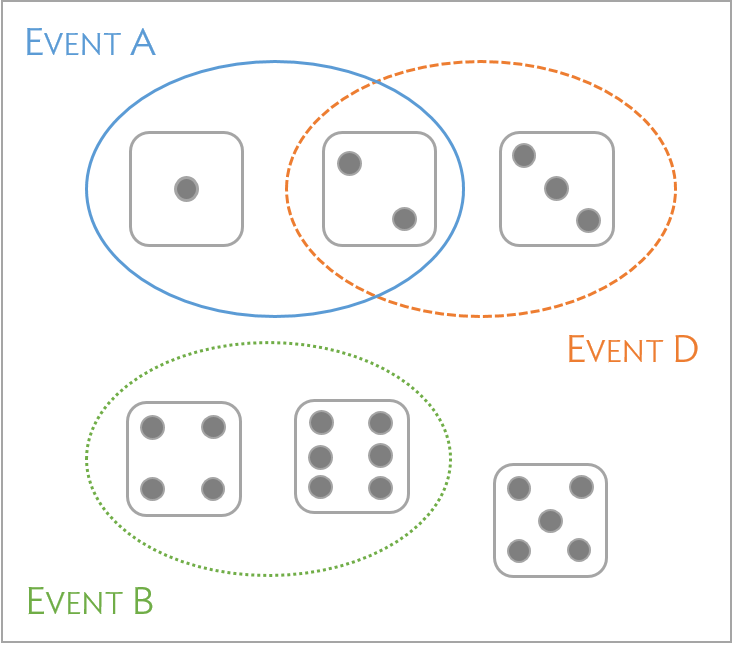
\includegraphics[width=2.5in]{figures/disjointEvents.png}
\end{center}

\end{frame}

\begin{frame}{Addition Rule for Disjoint Events}

If \(A\) and \(B\) represent two disjoint events, then the probability
that either occurs is \[P(A \cup B) = P(A) + P(B), \]

The \(\cup\) symbol denotes the \emph{union} of two events; i.e.,
\(P(A \text{ or } B)\).\footnote{Statistics uses the inclusive "or", such that $A$ or $B$ occurring means $A$, $B$, or both $A$ and $B$ occur.}

As shown on the previous slide, events \(A\) and \(B\) are disjoint.

\begin{itemize}
\item
  \(P(A \cup B) = P(A) + P(B) = 2/6 + 2/6 = 4/6\)
\item
  Intuitively, this makes sense; the probability of rolling either a 1,
  2, 4, or 6 on a six-sided die is 4/6.
\end{itemize}

If there are \(k\) disjoint events \(A_1,\dots,A_k\), then the
probability that one of these outcomes will occur is
\[P(A_1) + P(A_2) + \cdots + P(A_k)\]

\end{frame}

\begin{frame}{General Addition Rule}

Suppose that we are interested in the probability of drawing a diamond
or a face card out of a standard 52-card deck.

\begin{center}
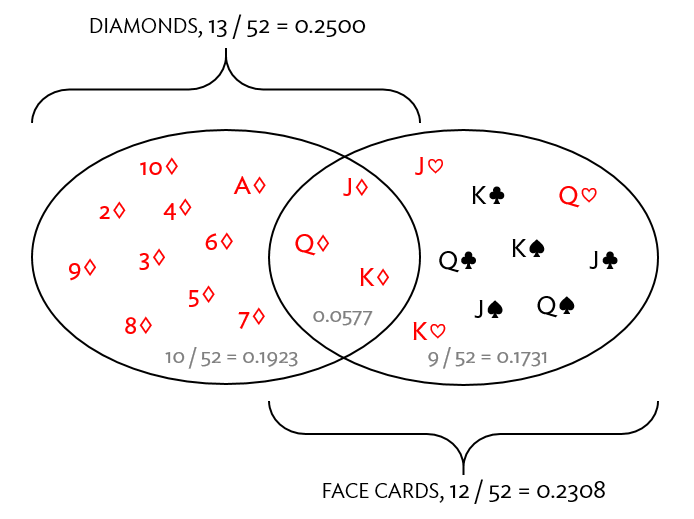
\includegraphics[width=2.5in]{figures/cardsDiamondFaceVenn.png}
\end{center}

Does \(P(\text{diamond or face card}) = 13/52 + 12/52\)?

\end{frame}

\begin{frame}{General Addition Rule\ldots{}}

To correct the double counting of the three cards that are in both
events, subtract the probability that both events occur\ldots{}

\begin{align*}
P(\text{diamond or face card}) =& P(\text{diamond}) + P(\text{face card}) - P(\text{diamond and face card}) \\
=& 13/52 + 12/52 - 3/52 \\
=& 22/52
\end{align*}

Thus, for any two events \(A\) and \(B\), the probability that either
occurs is \[P(A \cup B) = P(A) + P(B) - P(A \cap B).\]

The \(\cap\) symbol denotes the \emph{intersection} of two events; i.e.,
\(P(A \text{ and }B)\).

\end{frame}

\begin{frame}{Sample Space}

A \emph{sample space} is a list of exhaustive and mutually exclusive
outcomes.

Suppose the possible \(k\) outcomes are denoted
\(O_1, O_2, \dots, O_k\). The sample space can be expressed as
\(S = \{O_1, O_2, \dots, O_k\}\).

\begin{itemize}
\tightlist
\item
  For the die tossing experiment, \(S = \{1, 2, 3, 4, 5, 6\}\)
\end{itemize}

Given a sample space \(S = \{O_1, O_2, \dots, O_k\}\), the sum of the
probabilities of each outcome must equal 1.

\[\sum_{i=1}^{k}P(O_i)=1\]

\end{frame}

\begin{frame}{Complement of an Event}

Let \(D = \{2, 3\}\) represent the event that the outcome of a die roll
is 2 or 3.

The \emph{complement} of \(D\) represents all outcomes in the sample
space that are not in \(D\).

\begin{center}
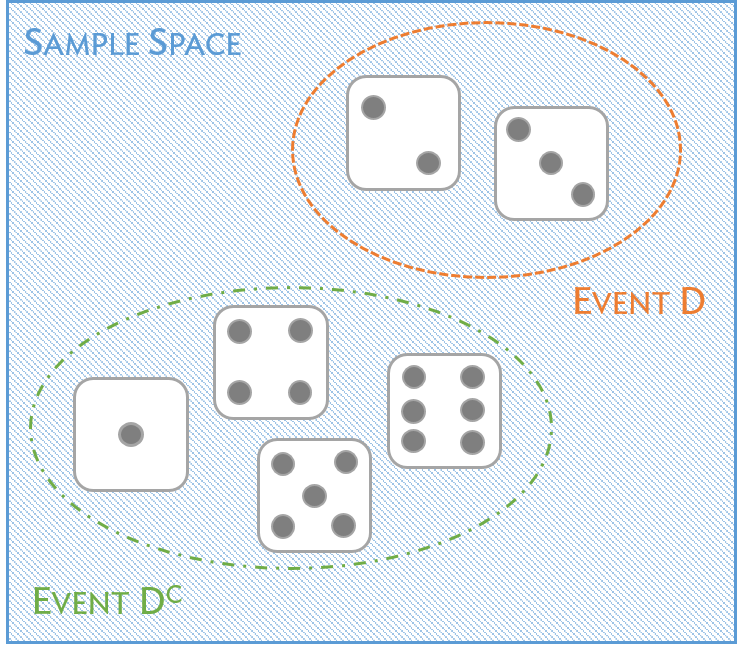
\includegraphics[width=2.5in]{figures/complementOfD.png}
\end{center}

\end{frame}

\begin{frame}{Complement of an Event\ldots{}}

The complement of an event \(A\) is denoted by \(A^C\).

An event and its complement are mathematically related:

\[P(A) + P(A^C) = 1 \qquad P(A) = 1 - P(A^C)\]

\end{frame}

\begin{frame}{Independent Events}

Two events \(A\) and \(B\) are \emph{independent} if the probability
that both \(A\) and \(B\) occur equal the product of their separate
probabilities.

\[P(A \cap B) = P(A)P(B) \]

\begin{center}
\begin{figure}
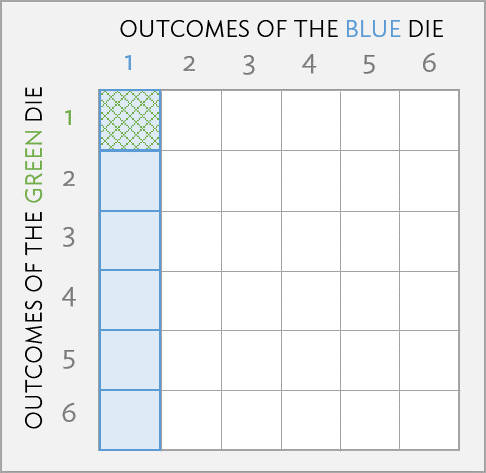
\includegraphics[width=1.5in]{figures/indepForRollingTwo1s.png}
\caption{A blue die and a green die are rolled. What is the probability of rolling two 1's?}
\end{figure}
\end{center}

\end{frame}

\section{Conditional Probability}\label{conditional-probability}

\begin{frame}{An example from childhood mortality}

\begin{center}
\begin{figure}
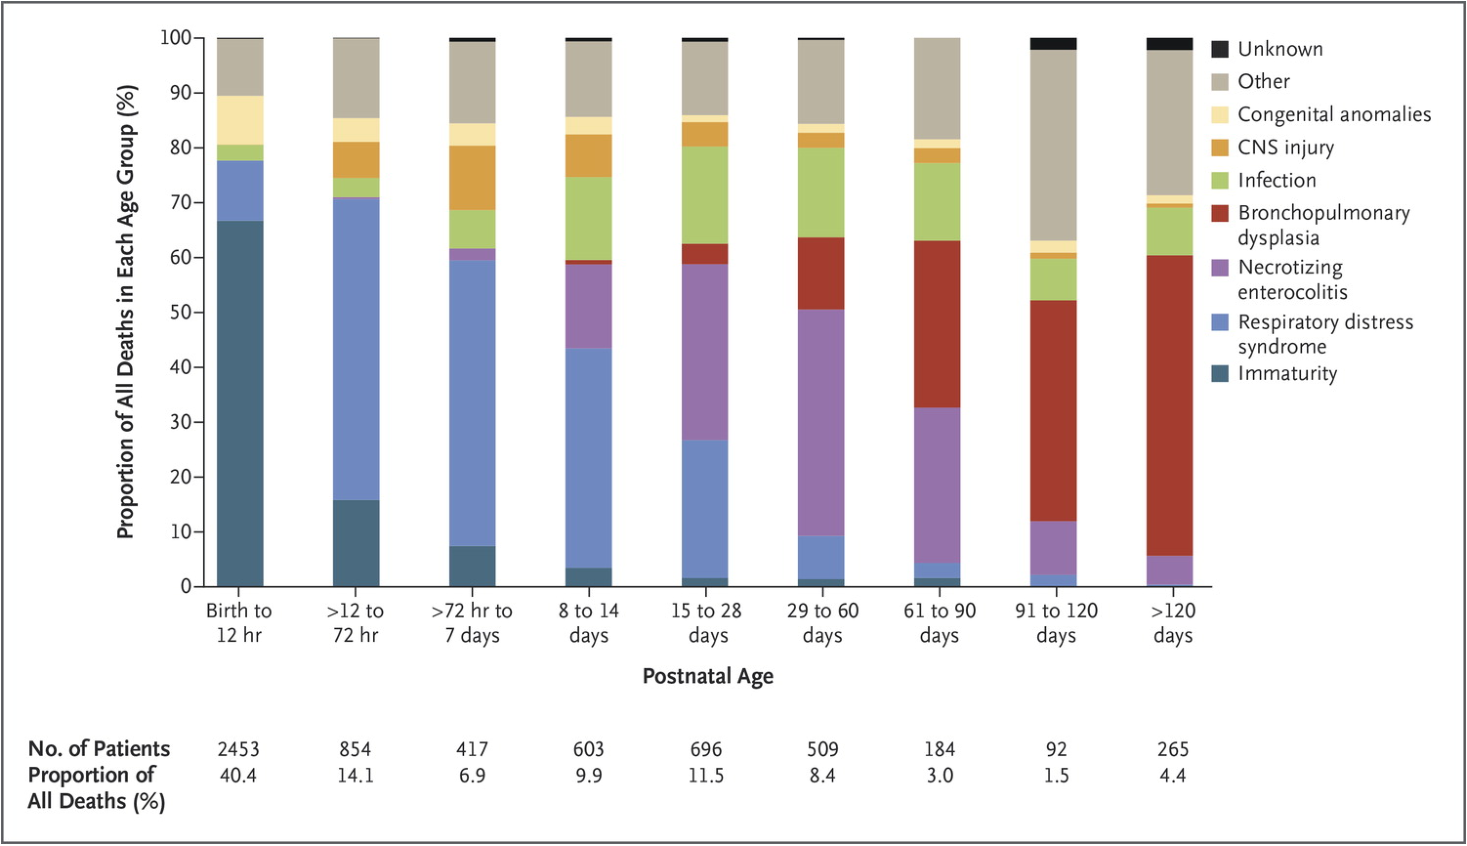
\includegraphics[width=4.5in]{figures/premature_infant_death}
\end{figure}
\end{center}

\footnotesize

Published in Patel, et al., \emph{NEJM} (2015) Vol 372, pp 331 - 340.

\end{frame}

\begin{frame}{Conditional Probability: Intuition}

Consider height in the US population.

What is the probability that a randomly selected individual in the
population is taller than 6 feet, 4 inches?

\begin{itemize}
\item
  Suppose you learn that the individual is a professional basketball
  player.
\item
  Does this change the probability that the individual is taller than 6
  feet, 4 inches?
\end{itemize}

\end{frame}

\begin{frame}{Conditional Probability: Concept}

The \textbf{conditional probability} of an event \(A\), given a second
event \(B\), is the probability of \(A\) happening, knowing that the
event \(B\) has happened.

\begin{itemize}
\tightlist
\item
  This conditional probability is denoted \(P(A|B)\).
\end{itemize}

Toss a fair coin three times. Let \(A\) be the event that \emph{exactly}
two heads occur, and \(B\) the event that \emph{at least} two heads
occur.

\begin{itemize}
\item
  \(P(A|B)\) is the probability of having exactly two heads among the
  outcomes that have at least two heads.
\item
  Conditioning on \(B\) means that the sample space consists of
  \(\{HHH, HHT, HTH, THH\}\), all possible sets of three tosses where at
  least two heads occurred.
\item
  In this set of outcomes, \(A\), consists of the last three, so
  \(P(A|B) = 3/4\).
\end{itemize}

\end{frame}

\begin{frame}{Conditional Probability: Formal Definition}

As long as \(P(B) > 0\), \[P(A|B) = \dfrac{P(A \cap B)}{P(B)}. \]

From the definition,

\begin{align*}
P(A|B) =& \dfrac{P(\text{at least two heads and exactly two heads})}{P(\text{at least two heads})} \\
=& \dfrac{P(\text{exactly two heads})}{P(\text{at least two heads})} \\
=& \dfrac{(3/8)}{(4/8)} = 3/4
\end{align*}

\end{frame}

\begin{frame}{Independence, Again\ldots{}}

A consequence of the definition of conditional probability:

\begin{itemize}
\tightlist
\item
  If \(P(A|B) = P(A)\), then \(A\) and \(B\) are independent; knowing
  \(B\) offers no information about whether \(A\) occurred.
\end{itemize}

\end{frame}

\begin{frame}{General Multiplication Rule}

If \(A\) and \(B\) represent two outcomes or events, then
\[P(A \cap B) = P(A|B)P(B).\]

This follows from rearranging the definition of conditional probability:
\[P(A|B) = \frac{P(A \cap B)}{P(B)} \rightarrow P(A|B)P(B) = P(A \cap B)\]

Unlike the previously mentioned multiplication rule, this is valid for
events that might not be independent.

\end{frame}

\section{Positive Predictive Value of a Diagnostic Test (Bayes'
Theorem)}\label{positive-predictive-value-of-a-diagnostic-test-bayes-theorem}

\begin{frame}{Pre-natal testing for trisomy 21, 13, and 18}

Some congenital disorders are caused by an additional copy of a
chromosome being attached (translocated) to another chromosome during
reproduction.

\begin{itemize}
\item
  Trisomy 21: Down syndrome, approximately 1 in 800 births
\item
  Trisomy 13: Patau's syndrome, physical and mental disabilities,
  approximately 1 in 16,000 newborns
\item
  Trisomy 18: Edward's syndrome, nearly always fatal, either in
  stillbirth or infant mortality. Occurs in about 1 in 6,000 births
\end{itemize}

Until recently, testing for these conditions consisted of screening the
mother's blood for serum markers, followed by amniocentesis in women who
test positive.

\end{frame}

\begin{frame}{Cell-free fetal DNA (cfDNA)}

cfDNA consists of copies of embryo DNA present in maternal blood.

Advances in sequencing DNA provided possibility of non-invasive testing
for these disorders, using only a blood sample.

Initial testing of the technology was done using archived samples of
genetic material from children whose trisomy status was known.

The results are variable, but generally very good:

\begin{itemize}
\item
  Of 1000 unborn children with the one of the disorders, approximately
  980 have cfDNA that tests positive. The test has high
  \emph{sensitivity}.
\item
  Of 1000 unborn children without the disorders, approximately 995 test
  negative. The test has high \emph{specificity}.
\end{itemize}

\end{frame}

\begin{frame}{Cell-free fetal DNA (cfDNA)\ldots{}}

The designers of a diagnostic test want the test to be accurate.

\begin{itemize}
\tightlist
\item
  In other words, the test should have high sensitivity and specificity.
\end{itemize}

A family with an unborn child undergoing testing, however, wants to know
the likelihood of the condition being present if the test is positive.

Suppose a child has tested positive for trisomy 21. What is the
probability that the child does have the trisomy 21 condition, given the
positive test result?

\end{frame}

\begin{frame}{Defining events in diagnostic testing}

Events of interest in diagnostic testing:

\begin{itemize}
\item
  \(D\) = \{disease present\}
\item
  \(D^C\) = \{disease absent\}
\item
  \(T^+\) = \{positive test result\}
\item
  \(T^-\) = \{negative test result\}
\end{itemize}

\vspace{0.5cm}

Could use \(T\) and \(T^C\), but \(T^+\) and \(T^-\) are consistent with
notation in medical and public health literature.

\end{frame}

\begin{frame}{Characteristics of a diagnostic test}

The following measures are all characteristics of a diagnostic test.

\begin{itemize}
\item
  Sensitivity = \(P (T^+ | D)\)
\item
  Specificity = \(P(T^- | D^C)\)
\item
  False negative rate = \(P(T^- | D)\)

  \begin{itemize}
  \tightlist
  \item
    Note that \(P(T^- | D) = 1 - P (T^+ | D)\), i.e., 1 - sensitivity
  \end{itemize}
\item
  False positive rate = \(P(T^+ | D^C)\)

  \begin{itemize}
  \tightlist
  \item
    Note that \(P(T^+ | D^C) = 1 - P (T^- | D^C)\), i.e., 1 -
    specificity
  \end{itemize}
\end{itemize}

\end{frame}

\begin{frame}{Positive predictive value of a test}

Suppose an individual tests positive for a disease.

The \textbf{positive predictive value (PPV)} of a diagnostic test is the
probability that a person has the disease, given that he/she has tested
positive for it.

\begin{itemize}
\tightlist
\item
  PPV = \(P(D | T^+)\)
\end{itemize}

The characteristics of a diagnostic test include \(P(T^+|D)\), among
other probabilities, but not the reverse conditional probability
\(P(D|T^+)\).

\end{frame}

\begin{frame}{Bayes' Theorem, aka Bayes' Rule}

Bayes' Thorem (simplest form):

\[ P(A|B) = \frac{P(B|A)P(A)}{P(B)}\]

Follows directly from the definition of conditional probability by
noting that \(P(A) P(B|A)\) equals \(P(A \text{ and } B)\):

\[P(A|B) =  \frac{P(A \cap B)}{P(B)} = \frac{P(B|A)P(A)}{P(B)}\]

\end{frame}

\begin{frame}{The denominator P(B) in Bayes' Theorem}

Bayes' Theorem is seldom stated in its simplest form, because in many
problems, \(P(B)\) is not given directly, but is calculated using the
general multiplication formula for probabilities:

Suppose \(A\) and \(B\) are events. Then,

\begin{align*}
P(B) = & P(B \cap A) + P(B \cap A^C) \\
    = & P(B | A)P(A)+ P(B|A^C)P(A^C)
\end{align*}

Bayes' Theorem can be written as:

\[P(A|B) = \frac{P(A) P(B|A)}{P(B)} = \frac{P (B|A)P(A)}{P (B | A)P(A) + P (B|A^C)P(A^C)} \]

\end{frame}

\begin{frame}{Bayes' Theorem for diagnostic tests}

\begin{align*}
  P(D|T^+) = & \dfrac{P(D \cap T^{+})}{P(T^+)} \\ 
  =& \dfrac{P(D \cap T^{+})}{P(D \cap T^{+}) + P(D^C \cap T^{+})} \\
  = & \frac{P(T^{+}|D)P(D)}{P(T^{+}|D)P(D)+
    P(T^{+}|D^{C})P(D^C)} \\
  = & \frac{\text{sensitivity} \times \text{prevalence}}{[\text{sensitivity} \times \text{prevalence}] + [(\text{1 - specificity}) \times (\text{1 - prevalence})]}  
\end{align*}

\end{frame}

\begin{frame}{Bayes' Theorem for diagnostic tests\ldots{}}

\begin{center}
\begin{figure}
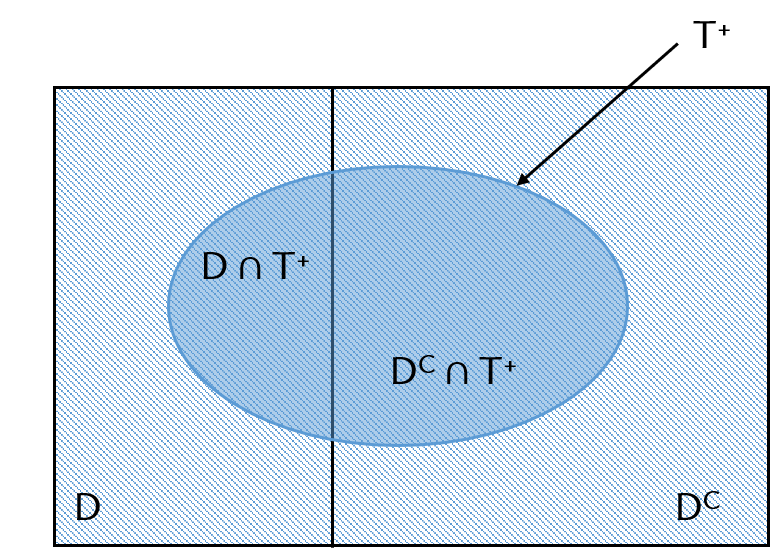
\includegraphics[width=3in]{figures/bayesVenn}
\end{figure}
\end{center}

\[P(D|T^+) = \dfrac{P(D \cap T^{+})}{P(T^+)} = \dfrac{P(D \cap T^{+})}{P(D \cap T^{+}) + P(D^C \cap T^{+})}\]

\end{frame}

\end{document}
